\documentclass[12pt]{article}
\usepackage[margin=2.5cm]{geometry}
\usepackage{enumerate}
\usepackage{amsfonts}
\usepackage{amsmath}
\usepackage{fancyhdr}
\usepackage{amsmath}
\usepackage{amssymb}
\usepackage{amsthm}
\usepackage{mdframed}
\usepackage{graphicx}
\usepackage{subcaption}
\usepackage{adjustbox}
\usepackage{listings}
\usepackage{xcolor}
\usepackage{booktabs}
\usepackage[utf]{kotex}

\definecolor{codegreen}{rgb}{0,0.6,0}
\definecolor{codegray}{rgb}{0.5,0.5,0.5}
\definecolor{codepurple}{rgb}{0.58,0,0.82}
\definecolor{backcolour}{rgb}{0.95,0.95,0.92}

\lstdefinestyle{mystyle}{
    backgroundcolor=\color{backcolour},
    commentstyle=\color{codegreen},
    keywordstyle=\color{magenta},
    numberstyle=\tiny\color{codegray},
    stringstyle=\color{codepurple},
    basicstyle=\ttfamily\footnotesize,
    breakatwhitespace=false,
    breaklines=true,
    captionpos=b,
    keepspaces=true,
    numbers=left,
    numbersep=5pt,
    showspaces=false,
    showstringspaces=false,
    showtabs=false,
    tabsize=1
}

\lstset{style=mystyle}

\begin{document}
\title{CSC148 Worksheet 12 Solution}
\author{Hyungmo Gu}
\maketitle

\section*{Question 1}
\begin{enumerate}[a.]
    \item

    \adjustbox{valign=t}{
        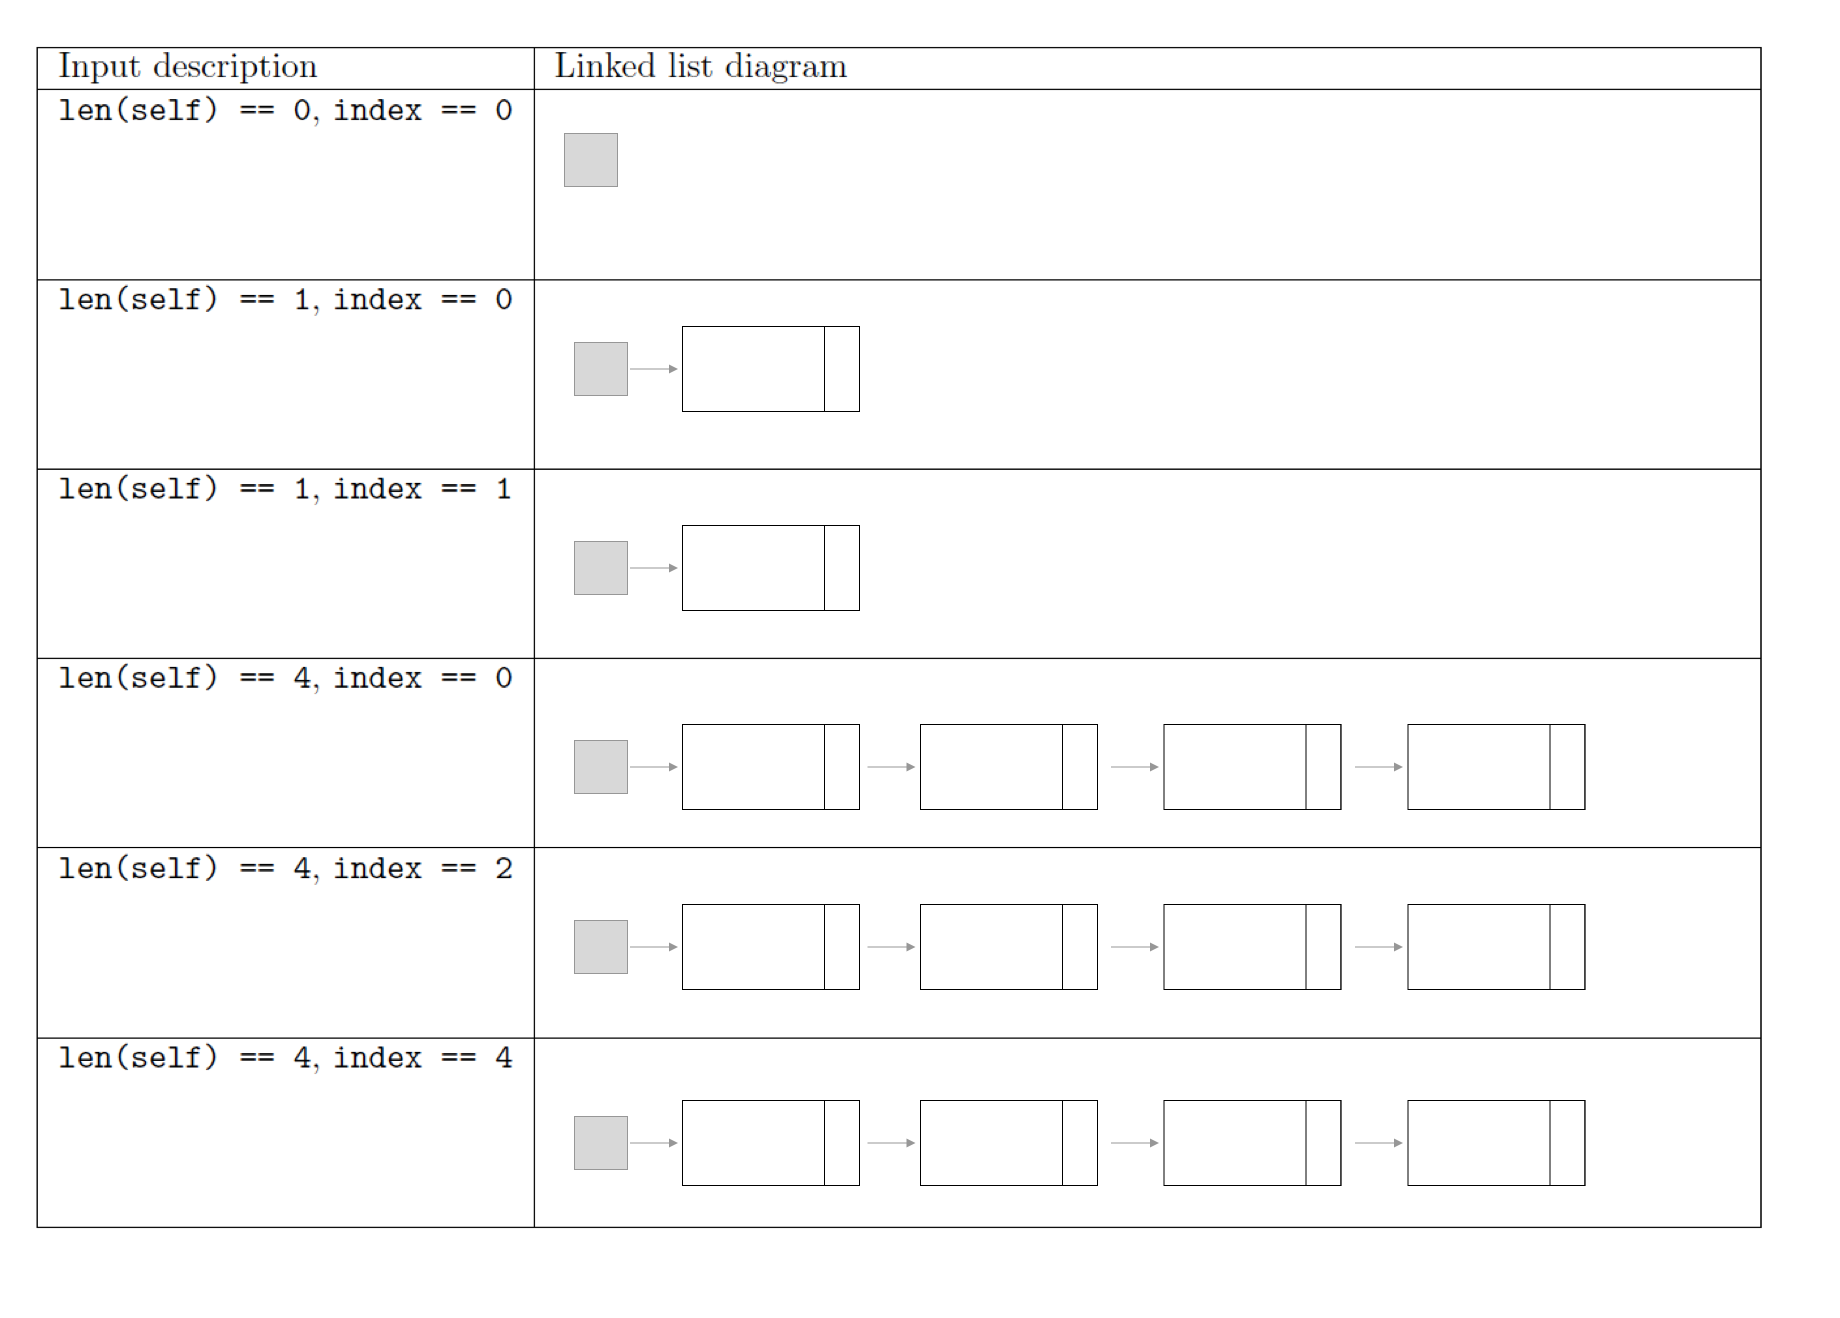
\includegraphics[width=\linewidth]{images/worksheet_12_q1a_solution.png}
    }

    \item

    \adjustbox{valign=t}{
        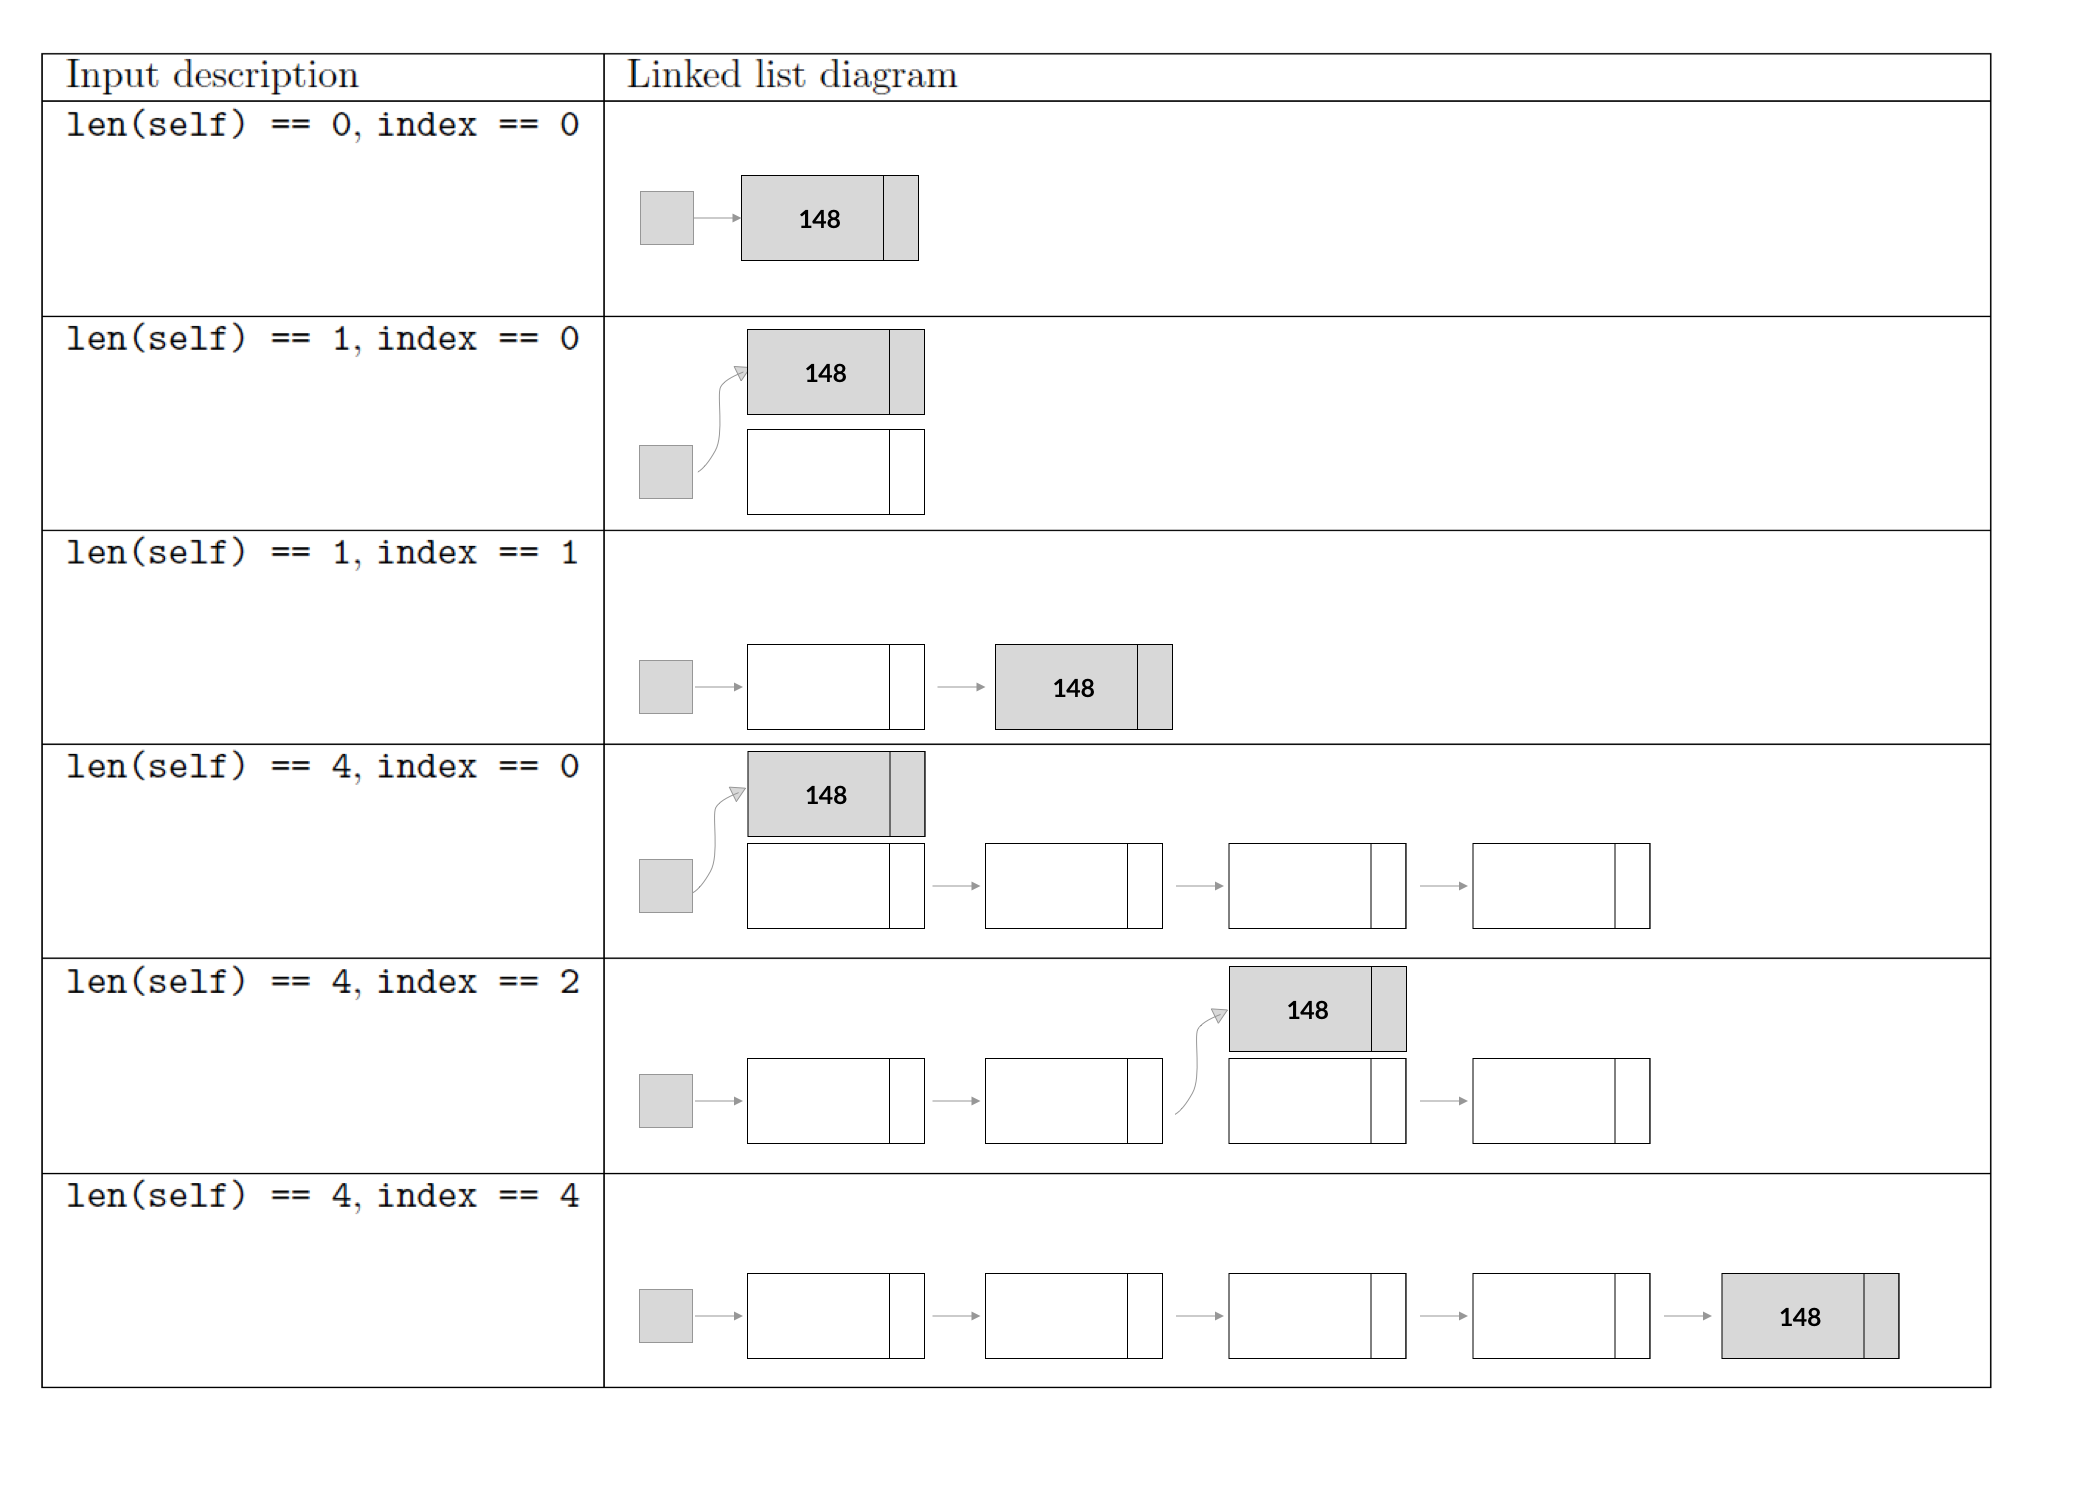
\includegraphics[width=\linewidth]{images/worksheet_12_q1b_solution.png}
    }

    \newpage

    \begin{mdframed}
        \underline{\textbf{Correct Solution:}}

        \bigskip

        \adjustbox{valign=t}{
            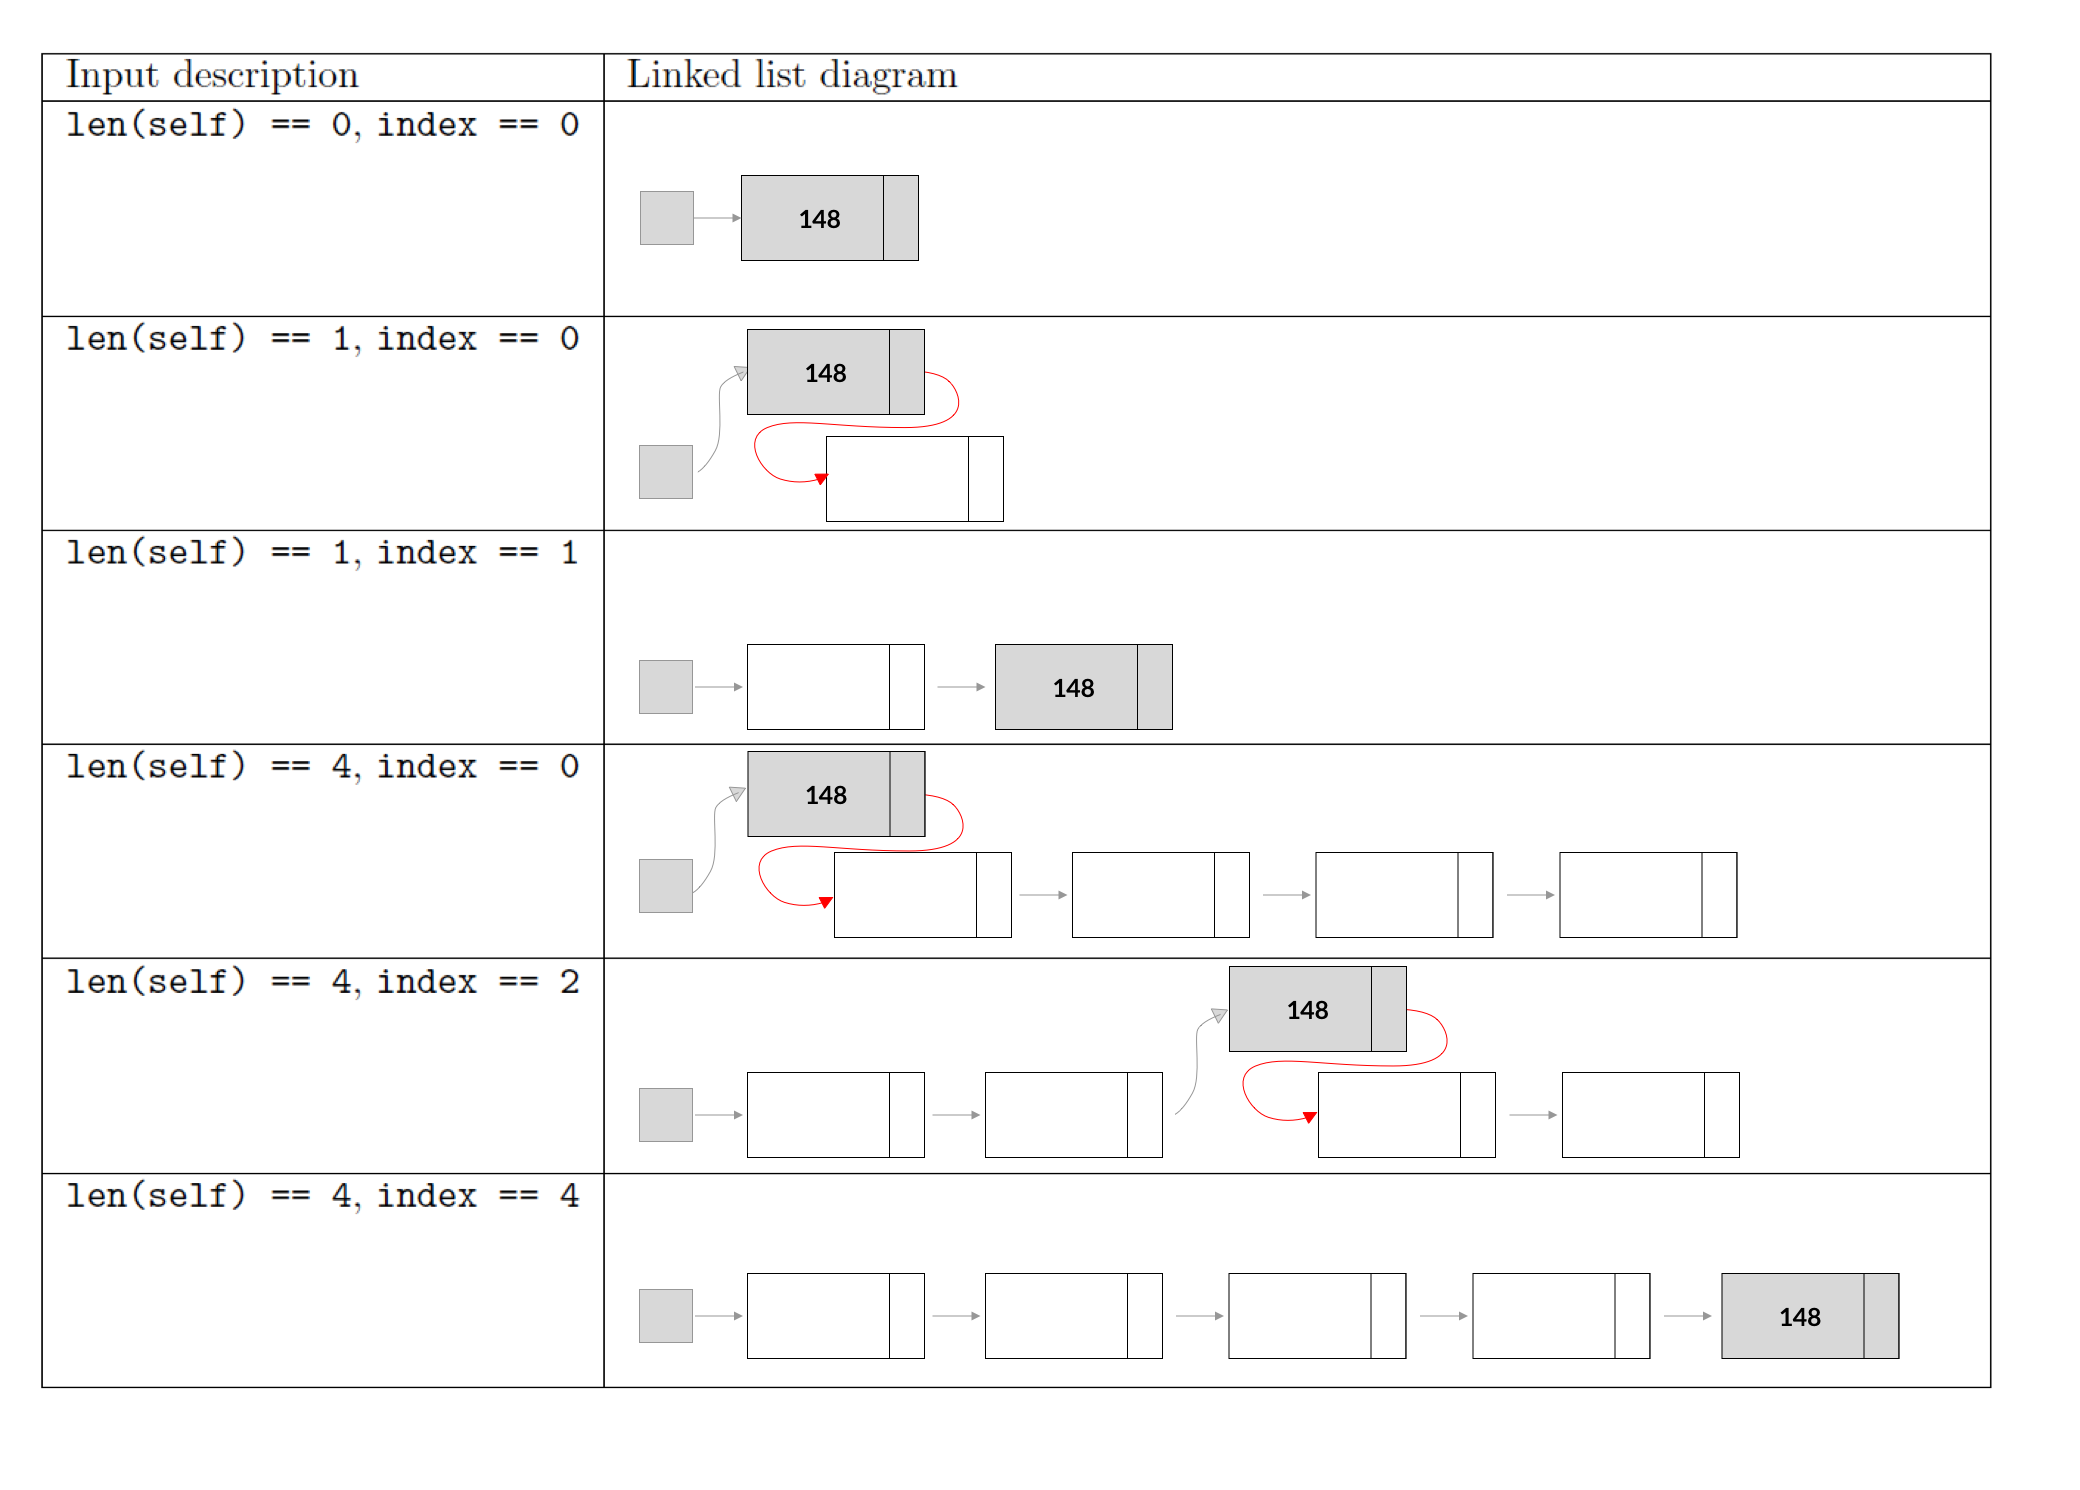
\includegraphics[width=\linewidth]{images/worksheet_12_q1b_correction.png}
        }
    \end{mdframed}

\end{enumerate}

\section*{Question 2}
\begin{enumerate}[a.]
    \item To reassign \textit{self.\_first} to something new, \textit{len(self)}
    can be value, but \textit{index} has to be at 0.

    \item To make \textit{insert} method to behave the same as \textit{LinkedList.append},
    \textit{len(self)} can be any value, but $index = len(self) - 1$.

    \bigskip

    \begin{mdframed}
        \underline{\textbf{Correct Solution:}}

        \bigskip

        To make \textit{insert} method to behave the same as \textit{LinkedList.append},
        \textit{len(self)} can be any value, but \color{red}$index = len(self)$\color{black}.
    \end{mdframed}

    \bigskip

    \underline{\textbf{Notes:}}

    \bigskip

    \begin{itemize}
        \item

        Learned that the first node in linked list represents $index = 0$.

        \begin{center}
        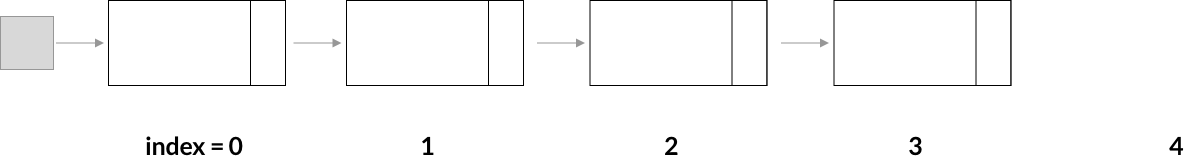
\includegraphics[width=\linewidth]{images/worksheet_12_q1b_note_1.png}
        \end{center}

        \item Learned that \textit{insert} operation for linked list is the same as
        the \textit{insert} operation for lists.

        \begin{itemize}
            \item If node doesn't exist at this index, then hook last node to the inserting node.
            \item If node does exist, then hook current node to one end of the
            inserting node, and the other end to the next node
        \end{itemize}
    \end{itemize}
\end{enumerate}

\section*{Question 3}
\begin{lstlisting}[language=Python,caption={worksheet\_12\_q3\_solution.py},captionpos=b]
    ...
    def insert(self, index: int, item: Any) -> None:
        """Insert a the given item at the given index in this list.
        Raise IndexError if index > len(self) or index < 0.
        Note that adding to the end of the list is okay.

        >>> lst = LinkedList([1, 2, 3])
        >>> lst.insert(0,0)
        >>> str(lst)
        '[0 -> 1 -> 2 -> 3]'
        >>> lst.insert(1,10)
        >>> str(lst)
        '[0 -> 10 -> 1 -> 2 -> 3]'
        >>> lst.insert(5,10)
        >>> str(lst)
        '[0 -> 10 -> 1 -> 2 -> 3 -> 10]'
        """

        curr = self._first
        current_index = 0

        if index == 0:
            current_node = curr
            self._first = _Node(item)
            self._first.next = current_node
            return

        while curr is not None:
            if current_index != index - 1:
                curr = curr.next
                current_index += 1
                continue

            # 1. if index == len(self), then append to list
            # 2. if index < len(self), then insert value at index
            current_node = curr.next
            inserting_node = _Node(item)
            curr.next = inserting_node
            inserting_node.next = current_node
            return

        # 3. if index > len(self), raise IndexError
        raise IndexError
    ...
\end{lstlisting}

\end{document}